\chapter{Chapitre 4 : Réalisation et mise en pied du système}
\thispagestyle{fancy}
\newpage

\section{Outils et technologies de développement}
Pour le développement du projet, plusieurs outils et technologies modernes ont été utilisés afin d'assurer la qualité, la performance et la maintenabilité du code.

\subsection{Environnement de développement}
L'environnement de développement a été configuré avec les outils suivants :
\begin{itemize}
  \item \textbf{Visual Studio Code :} Comme éditeur de code principal avec des extensions pour React, TypeScript et ESLint
  \item \textbf{GitHub :} Pour la gestion de versions et la collaboration
  \item \textbf{Docker :} Pour la conteneurisation des services backend
  \item \textbf{Postman :} Pour tester les API
  \item \textbf{Chrome DevTools :} Pour le debugging et l'optimisation des performances frontend
\end{itemize}

\subsection{Technologies frontend}
Pour le développement front-end de cette application, les technologies suivantes ont été utilisées :
\begin{itemize}
  \item \textbf{Next.js :} Framework React pour le rendu côté serveur et la génération de sites statiques
  \item \textbf{Tailwind CSS :} Framework CSS utilitaire pour un design responsive et personnalisable
  \item \textbf{Framer Motion :} Bibliothèque d'animations pour ajouter des transitions et effets visuels
  \item \textbf{React Hook Form :} Gestion des formulaires avec validation
  \item \textbf{TypeScript :} Pour un code plus robuste avec typage statique
\end{itemize}

\subsection{Technologies backend}
Pour le développement backend, les technologies suivantes ont été utilisées :
\begin{itemize}
  \item \textbf{Node.js :} Environnement d'exécution JavaScript côté serveur
  \item \textbf{Express :} Framework web pour Node.js
  \item \textbf{PostgreSQL :} Système de gestion de base de données relationnelle
  \item \textbf{Supabase :} Plateforme Backend-as-a-Service pour l'authentification et le stockage
  \item \textbf{Redis :} Pour la mise en cache et la gestion des sessions
\end{itemize}

\section{Préparation de l'environnement de travail}
Avant de commencer le développement proprement dit, une phase de préparation de l'environnement a été nécessaire.

\subsection{Installation de XAMPP}
Pour faciliter le développement local, XAMPP a été installé comme solution tout-en-un comprenant Apache, MySQL, PHP et Perl. Les étapes d'installation ont inclus :
\begin{itemize}
  \item Téléchargement de la dernière version de XAMPP
  \item Installation et configuration des ports
  \item Configuration des droits d'accès et des répertoires virtuels
  \item Tests de fonctionnement du serveur local
\end{itemize}

\subsection{Installation de Laravel}
Après la mise en place de XAMPP, l'installation du framework Laravel a été effectuée :
\begin{itemize}
  \item Installation de Composer comme gestionnaire de dépendances PHP
  \item Installation globale de Laravel via Composer
  \item Création du projet avec la commande `composer create-project laravel/laravel`
  \item Configuration de la base de données dans le fichier `.env`
  \item Installation des dépendances supplémentaires nécessaires au projet
\end{itemize}

\section{Réalisation du site web}

\subsection{Développement de la Page d'Accueil}
La page d'accueil a été conçue pour présenter clairement la valeur ajoutée de la plateforme et inciter les utilisateurs à s'inscrire. Plusieurs sections ont été développées pour structurer l'information de manière efficace.

\begin{figure}[h!]
  \centering
  
\includegraphics[width=0.9\textwidth,keepaspectratio]{week_2_img/last_and_improved_hero_section_withe_3d_effects_etc.png}
  \caption{\textbf{Hero Section améliorée} de la page d'accueil avec effets 3D et animations interactives.}
  \label{fig:hero_section_improved}
\end{figure}

Les éléments clés de cette section comprennent :
\begin{itemize}
  \item Un titre accrocheur qui met en avant la proposition de valeur principale
  \item Un sous-titre explicatif sur les avantages de la plateforme
  \item Un bouton d'appel à l'action bien visible pour l'inscription
  \item Une illustration moderne avec des effets 3D représentant le concept d'apprentissage en ligne
  \item Un design responsive qui s'adapte à tous les types d'écrans
  \item Des animations interactives qui s'activent au survol ou au défilement
\end{itemize}

\begin{figure}[h!]
  \centering
  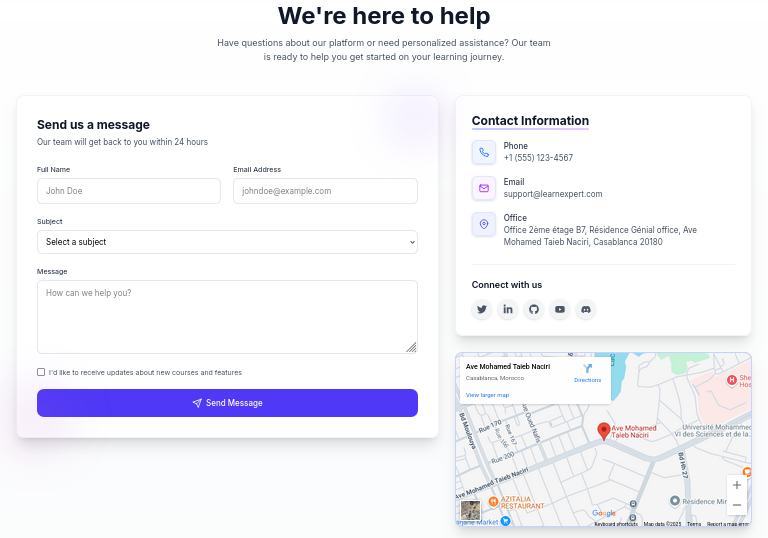
\includegraphics[width=0.9\textwidth,keepaspectratio]{week_2_img/where_we_are_section.png}
  \caption{\textbf{Section "Where We Are"} présentant la présence globale de la plateforme.}
  \label{fig:where_we_are}
\end{figure}

\begin{figure}[h!]
  \centering
  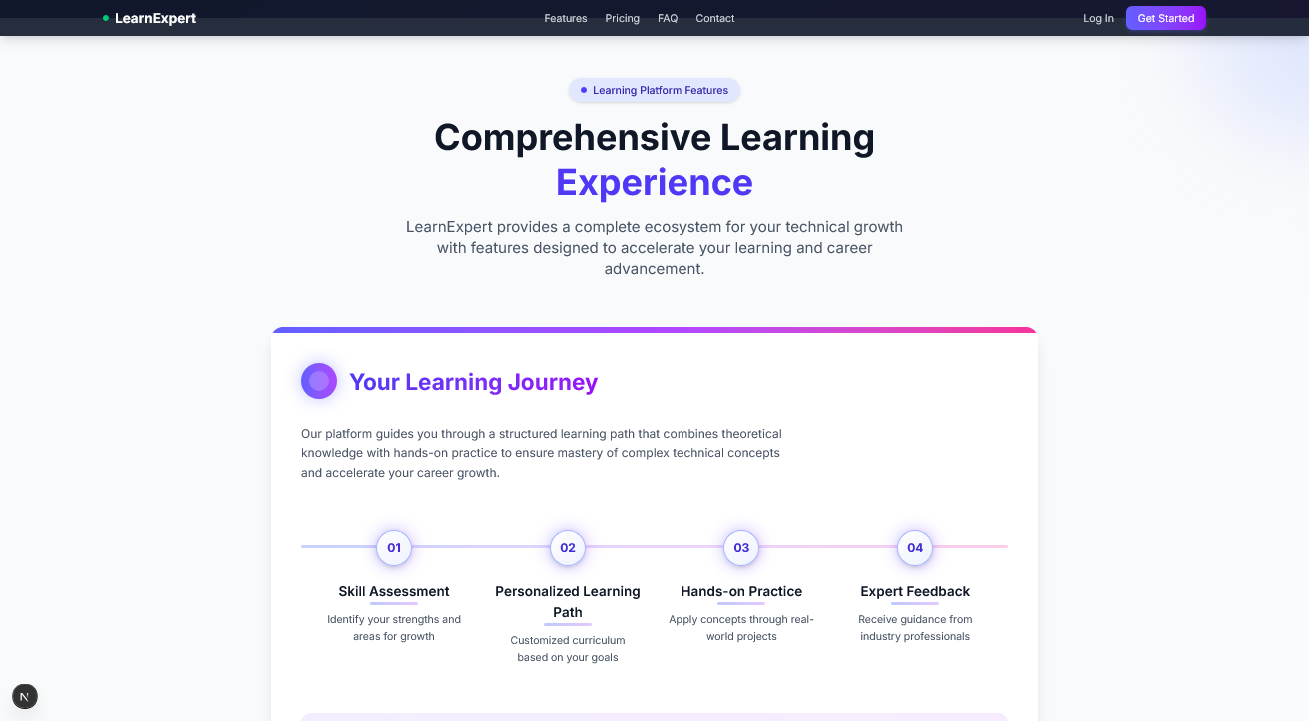
\includegraphics[width=0.9\textwidth,keepaspectratio]{week_2_img/featchersection_1.png}
  \caption{\textbf{Première section de fonctionnalités} présentant les cours en ligne.}
  \label{fig:features_section_1}
\end{figure}

\begin{figure}[h!]
  \centering
  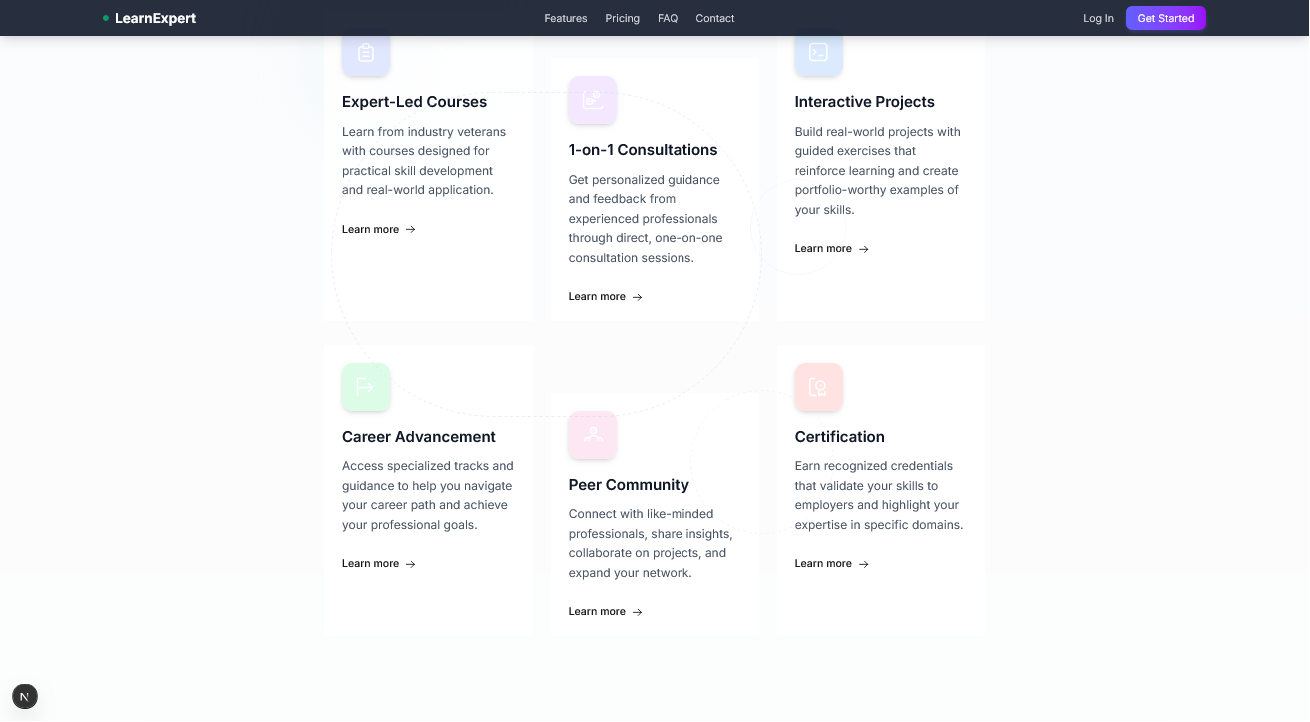
\includegraphics[width=0.9\textwidth,keepaspectratio]{week_2_img/fetchersection_2.png}
  \caption{\textbf{Deuxième section de fonctionnalités} mettant en avant les services de consultation.}
  \label{fig:features_section_2}
\end{figure}

\begin{figure}[h!]
  \centering
  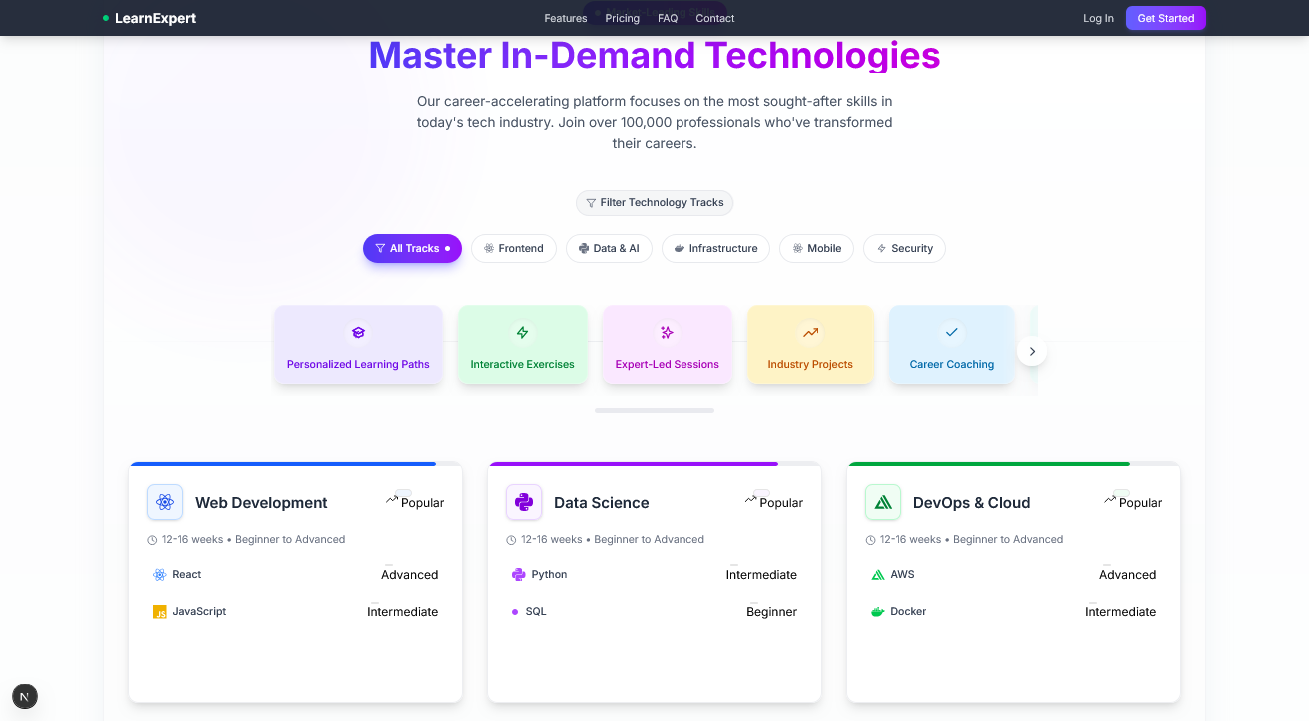
\includegraphics[width=0.9\textwidth,keepaspectratio]{week_2_img/fetchersection_3.png}
  \caption{\textbf{Troisième section de fonctionnalités} présentant les outils d'analyse et de suivi.}
  \label{fig:features_section_3}
\end{figure}

\subsection{Interface Utilisateur}
L'interface utilisateur a été développée en suivant les principes de conception centrée sur l'utilisateur :

\begin{figure}[h!]
  \centering
  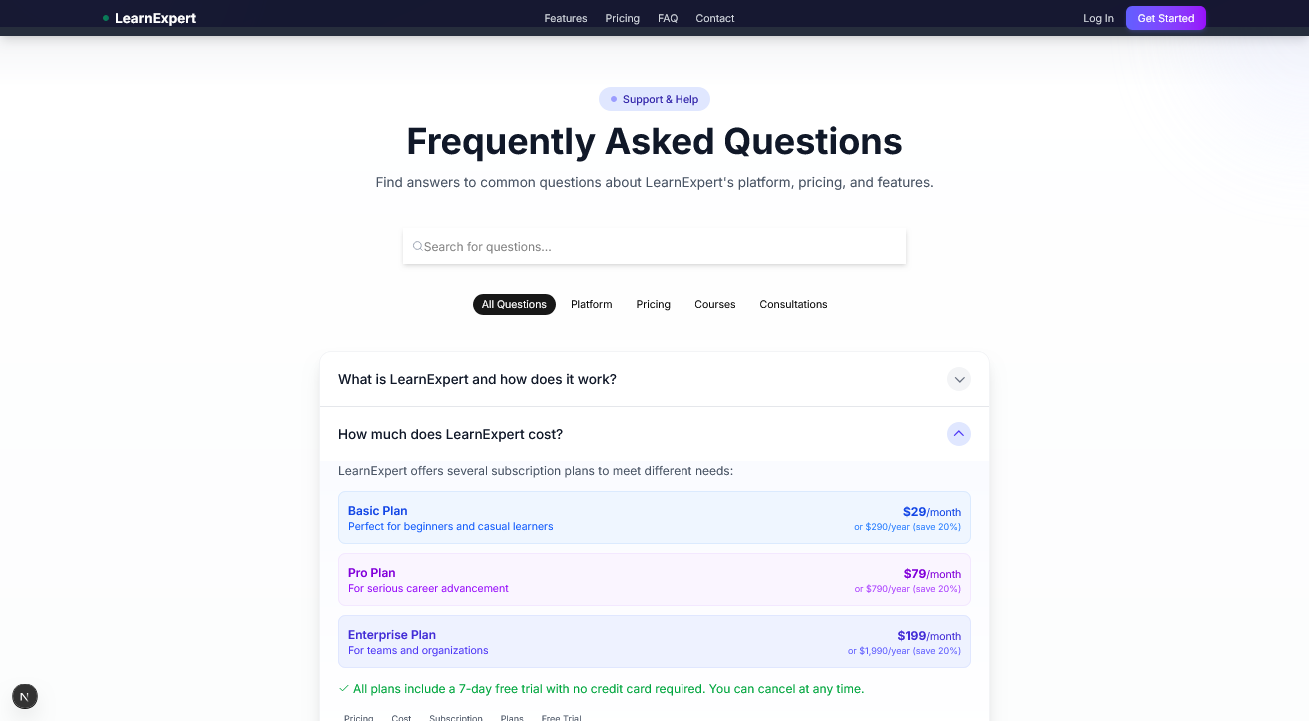
\includegraphics[width=0.9\textwidth,keepaspectratio]{week_2_img/faqsection.png}
  \caption{\textbf{Section FAQ} avec questions-réponses interactives.}
  \label{fig:faq_section}
\end{figure}

\begin{figure}[h!]
  \centering
  
\includegraphics[width=0.9\textwidth,keepaspectratio]{week_2_img/second_call_of_action.png}
  \caption{\textbf{Section d'appel à l'action finale} incitant à l'inscription.}
  \label{fig:final_cta}
\end{figure}

\begin{figure}[h!]
  \centering
  
\includegraphics[width=0.9\textwidth,keepaspectratio]{week_2_img/navbar.png}
  \caption{\textbf{Barre de navigation} avec les liens vers les principales sections.}
  \label{fig:navbar}
\end{figure}

\begin{figure}[h!]
  \centering
  
\includegraphics[width=0.9\textwidth,keepaspectratio]{week_2_img/foter.png}
  \caption{\textbf{Pied de page} avec informations légales et liens supplémentaires.}
  \label{fig:footer}
\end{figure}

\subsection{Intégration du Système de Paiement}
Un système de paiement sécurisé a également été intégré à la plateforme pour permettre l'achat d'abonnements et de services.

\begin{figure}[h!]
  \centering
  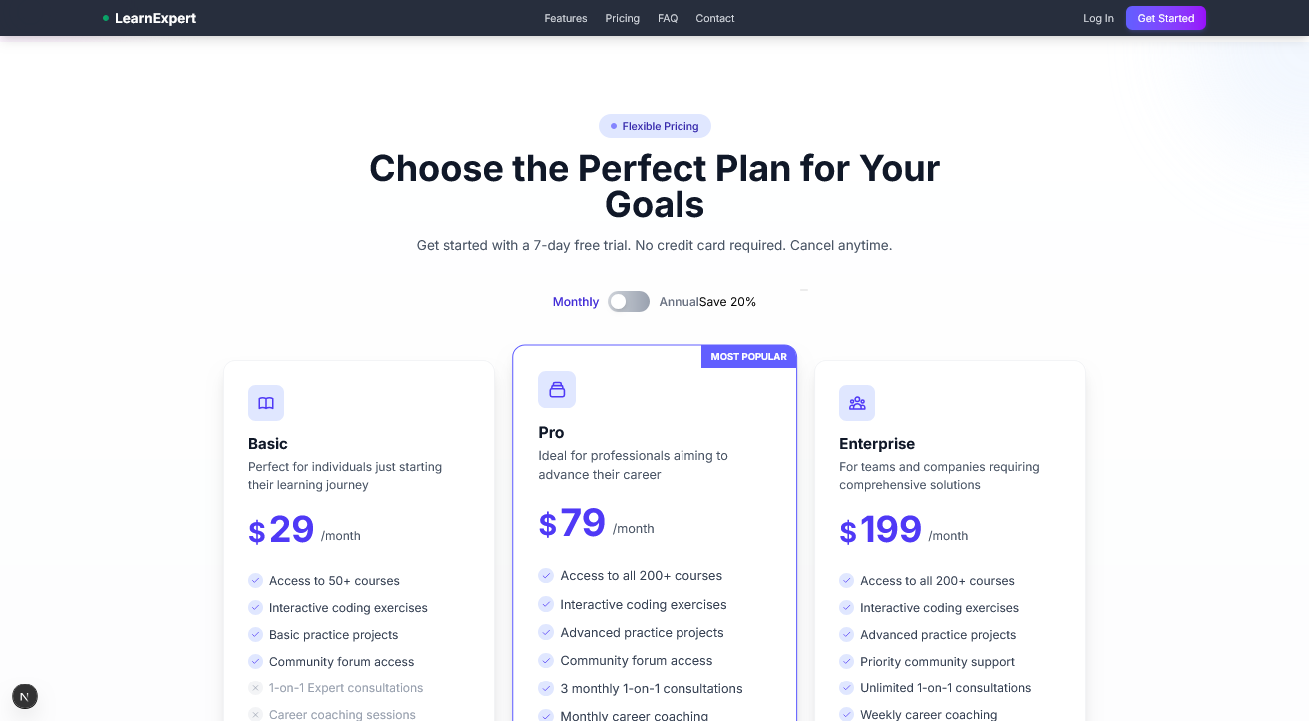
\includegraphics[width=0.9\textwidth,keepaspectratio]{week_2_img/payment_1.png}
  \caption{\textbf{Interface de paiement} pour les abonnements et services.}
  \label{fig:payment}
\end{figure}

Les fonctionnalités clés du système de paiement incluent :
\begin{itemize}
  \item Sélection de différentes formules d'abonnement
  \item Interface de saisie des informations de carte bancaire sécurisée
  \item Intégration avec un service de paiement externe (Stripe)
  \item Confirmation de paiement et génération de facture automatique
  \item Gestion des abonnements récurrents et des annulations
\end{itemize}

\subsection{Optimisations et Tests}
Une attention particulière a été portée à l'optimisation des performances :
\begin{itemize}
  \item Utilisation de l'optimisation d'images intégrée à Next.js
  \item Lazy loading des images et composants non critiques
  \item Minification du code CSS et JavaScript
  \item Mise en cache efficace pour réduire les temps de chargement
  \item Design responsive optimisé pour tous les appareils
  \item Tests de compatibilité sur différents navigateurs
  \item Tests de performance avec Lighthouse
\end{itemize}

\section{Méthodologie de Conception}

Le processus de conception de l'interface a suivi une approche méthodique :

\subsection{Analyse des Besoins et Recherche}
\begin{itemize}
  \item Étude des plateformes concurrentes pour identifier les meilleures pratiques
  \item Analyse des besoins des utilisateurs cibles
  \item Définition des objectifs principaux de la page d'accueil
\end{itemize}

\subsection{Wireframing et Prototypage}
\begin{itemize}
  \item Création de wireframes simples pour définir la structure de la page
  \item Développement de prototypes interactifs avec Figma
  \item Tests utilisateurs préliminaires pour valider les concepts
\end{itemize}

\subsection{Développement Itératif}
\begin{itemize}
  \item Implémentation progressive des différentes sections
  \item Sessions quotidiennes de feedback avec l'équipe
  \item Améliorations continues basées sur les retours
\end{itemize}

\section{Résultats et Impacts}

La conception de cette interface d'accueil a établi une base solide pour le développement des autres composants de la plateforme e-learning, en définissant une identité visuelle cohérente et en présentant clairement la proposition de valeur aux utilisateurs potentiels. 

\section{Conclusion}

Cette deuxième semaine de stage a été très productive, avec des avancées significatives dans le développement frontend de la plateforme. La création d'une page d'accueil attrayante et fonctionnelle constitue une étape importante du projet. Les différentes sections développées (Hero Section améliorée, Where We Are, fonctionnalités, FAQ, etc.) permettent de présenter efficacement la valeur ajoutée de la plateforme et d'inciter les utilisateurs à s'inscrire. Les prochaines étapes se concentreront sur le développement des interfaces internes pour les utilisateurs connectés et l'intégration des fonctionnalités backend. 